\documentclass[border=10pt]{standalone}
\usepackage[T1]{fontenc}
\usepackage{tikz}
\usetikzlibrary{positioning, arrows.meta, calc}

\definecolor{accent}{HTML}{1E3A8A}
\definecolor{boxfill}{HTML}{F1F5F9}
\definecolor{boxstroke}{HTML}{475569}

\begin{document}
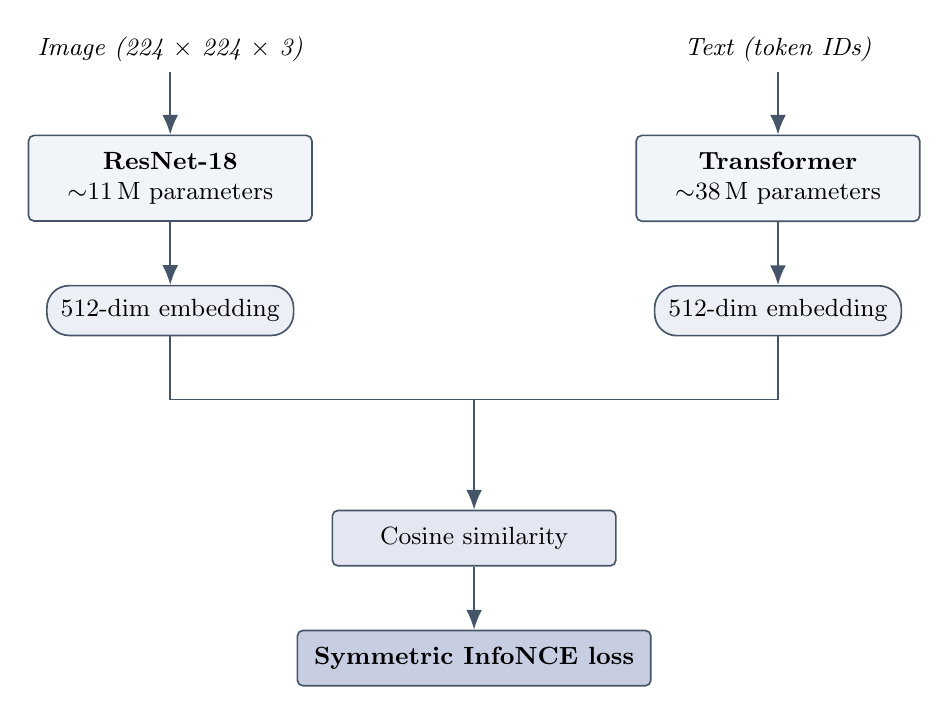
\begin{tikzpicture}[
  every node/.style={font=\small},
  >={Latex[length=2.5mm, width=2mm]},
  box/.style={
    draw=boxstroke, line width=0.6pt, fill=boxfill,
    rounded corners=2pt, inner sep=6pt,
    minimum width=36mm, align=center
  },
  pill/.style={
    draw=boxstroke, line width=0.6pt, fill=accent!8,
    rounded corners=8pt, inner sep=5pt,
    minimum width=26mm, align=center
  },
  arrow/.style={->, line width=0.6pt, draw=boxstroke}
]

% Inputs
\node[font=\small\itshape] (img) {Image (224 $\times$ 224 $\times$ 3)};
\node[font=\small\itshape, right=46mm of img] (txt) {Text (token IDs)};

% Encoders
\node[box, below=8mm of img] (resnet) {\textbf{ResNet-18}\\\small$\sim$11\,M parameters};
\node[box, below=8mm of txt] (xfmr)   {\textbf{Transformer}\\\small$\sim$38\,M parameters};

% Embeddings
\node[pill, below=8mm of resnet] (emb1) {512-dim embedding};
\node[pill, below=8mm of xfmr]   (emb2) {512-dim embedding};

% Convergence point
\coordinate (merge) at ($(emb1.south)!0.5!(emb2.south) + (0, -8mm)$);

% Cosine + loss
\node[box, below=14mm of merge, fill=accent!12] (sim) {Cosine similarity};
\node[box, below=8mm of sim, fill=accent!25] (loss) {\textbf{Symmetric InfoNCE loss}};

% Arrows
\draw[arrow] (img) -- (resnet);
\draw[arrow] (txt) -- (xfmr);
\draw[arrow] (resnet) -- (emb1);
\draw[arrow] (xfmr) -- (emb2);
\draw[line width=0.6pt, draw=boxstroke] (emb1.south) |- (merge);
\draw[line width=0.6pt, draw=boxstroke] (emb2.south) |- (merge);
\draw[arrow] (merge) -- (sim);
\draw[arrow] (sim) -- (loss);

\end{tikzpicture}
\end{document}
